% Machine translated from the Danish original, ../danish/ad-problems-june-2026.tex
\noindent\emph{This problem set has been machine translated from the Danish original.}
\medskip

\section*{Multiple-choice}\label{sec:mc}

\placeholder{Where to enter the multiple-choice answers, e.g.\ the multiple-choice module of the exam system.}

\multiplechoicestart

\question{MergeSort and comparisons}
Consider the following input to {\sc MergeSort}, implemented as in CLRS Section 2.3.
\begin{center}
\begin{tabular}{|c|c|c|c|}
\hline
4 & 3 & 1 & 2\\
\hline
\end{tabular}
\end{center}
How many comparisons between two elements does {\sc MergeSort} make in total on this input?
Comparisons with $\infty$ in {\sc Merge} are not counted.
\oneanswer
\optionsstart
\answer 3 comparisons are made
\answer 4 comparisons are made\correct
\answer 5 comparisons are made
\answer 6 comparisons are made
\answer 7 comparisons are made
\optionsend
\explanation{
The two recursive calls on the lists $\langle 4,3\rangle$ and $\langle 1,2\rangle$ each use one comparison.
After these calls, the sorted lists $\langle 3,4\rangle$ and $\langle 1,2\rangle$ are merged.
This merge uses two comparisons: $3$ against $1$ and then $3$ against $2$.
In total, $1+1+2=4$ comparisons are therefore used.
}


\question{Asymptotic bounds}
Which of the running times below are $O(n^2)$?
\multipleanswers
\optionsstart
\answer{$2^{\lg n}$}\correct
\answer{$n^3$}
\answer{$1.5^n$}
\answer{$\sqrt{n}$}\correct
\answer{$\lg n$}\correct
\optionsend
\explanation{
We check whether each function grows at most quadratically.
$2^{\lg n} = n$, since $\lg n = \log_2 n$, and therefore $2^{\lg n} = n$. Hence the function is also $O(n^2)$.
In contrast, $n^3$ grows faster than $n^2$ and is therefore not $O(n^2)$.
$1.5^{n}$ grows faster than any polynomial in~$n$, including $n^2$, and is therefore not $O(n^2)$.
Finally, $\sqrt{n} = n^{1/2}$ and $\log n$ both grow asymptotically slower than $n^2$, so they are $O(n^2)$.
}


\question{Solving recurrences}
Assume that $n$ is a power of 2, that $T_i(1)=1$ for $i=1,\dots,6$, and consider the recurrences below. Which of the following statements are true?
\multipleanswers
\optionsstart
\answer $T_1(n) = 2\,T_1(n/2) + n \log n$ has solution $T_1(n) = \Theta(n \log n)$.
\answer $T_2(n) = 4\,T_2(n/4) + n^2$ has solution $T_2(n) = \Theta(n^2)$.\correct
\answer $T_3(n) = 4\,T_3(n/2) + n$ has solution $T_3(n) = \Theta(n^2)$.\correct
\answer $T_4(n) = 4\,T_4(n/2) + n^2$ has solution $T_4(n) = \Theta(n^2)$.
\answer $T_5(n) = 8\,T_5(n/2) + n^2 \log n$ has solution $T_5(n) = \Theta(n^3)$.\correct
\answer $T_6(n) = 8\,T_6(n/2) + n^3$ has solution $T_6(n) = \Theta(n^3)$.
\optionsend
\explanation{The master theorem can be used to find a solution to all of the recurrences:
Write $T(n)=aT(n/b)+f(n)$ and compare $f(n)$ with $n^{\log_b a}$.
\begin{enumerate}
    \item $a=2,b=2$: $n^{\log_b a}=n$, and $f(n)=n\log n=\Theta(n^{\log_b a}\log n)$, so $T_1(n)=\Theta(n\log^2 n)$ (the statement is false).
\item $a=4,b=4$: $n^{\log_b a}=n$, and $f(n)=n^2=\Omega(n^{1+\varepsilon})$ with the regularity condition $af(n/b)=4(n/4)^2=n^2/4\le c n^2$, so $T_2(n)=\Theta(n^2)$ (true).
\item $a=4,b=2$: $n^{\log_b a}=n^2$, and $f(n)=n=O(n^{2-\varepsilon})$, so $T_3(n)=\Theta(n^2)$ (true).
\item $a=4,b=2$: $n^{\log_b a}=n^2$, and $f(n)=n^2=\Theta(n^{\log_b a})$, so $T_4(n)=\Theta(n^2\log n)$ (false).
\item $a=8,b=2$: $n^{\log_b a}=n^3$, and $f(n)=n^2 \log n = O(n^{3-\varepsilon})$, so $T_5(n)=\Theta(n^3)$ (true).
\item $a=8,b=2$: $n^{\log_b a}=n^3$, and $f(n)=n^3=\Theta(n^{\log_b a})$, so $T_6(n)=\Theta(n^3\log n)$ (false).
\end{enumerate}
}


\question{Setting up a recurrence}
Consider the following recursive algorithm:
\begin{codebox}
  \Procname{$\proc{RecursiveMystery}(A,i,j)$}
  \li \If $i \ge j$
  \li \Then
        \Return $0$
      \End
  \li $q \gets \lfloor (i+j)/2 \rfloor$
  \li $x \gets \proc{RecursiveMystery}(A,i,q)$
  \li $y \gets \proc{RecursiveMystery}(A,q+1,j)$
  \li $c \gets 0$
  \li \For $p \gets i$ \To $q$
  \li \Do
        \For $r \gets q+1$ \To $j$
  \li   \Do
          \If $A[p] = A[r]$
  \li     \Then
            $c \gets c+1$
          \End
        \End
      \End
  \li \Return $x+y+c$
\end{codebox}
Assume that \(n\) is a power of 2 and that all elementary operations take constant time.
Which recurrence best describes the running time \(T(n)\) of the following call?
\[
\proc{RecursiveMystery}(A,1,n)
\]
\oneanswer
\optionsstart
\answer \(T(n)=T(n/2)+\Theta(n)\)
\answer \(T(n)=T(n/2)+\Theta(n^2)\)
\answer \(T(n)=2T(n/2)+\Theta(n)\)
\answer \(T(n)=2T(n/2)+\Theta(n^2)\) \correct
\answer \(T(n)=3T(n/2)+\Theta(n)\)
\answer \(T(n)=3T(n/2)+\Theta(n^2)\)
\optionsend

\explanation{
For \(n>1\) the algorithm makes two recursive calls, and each call works on one half of the array, with input size \(n/2\).
This contributes \(2T(n/2)\).
After the recursive calls, the two nested loops count the number of pairs of equal elements where one element lies in the left half and the other in the right half.
There are \((n/2)\cdot(n/2)=\Theta(n^2)\) such pairs, and the test and any increment take constant time for each pair.
The running time is therefore described by
\[
T(n)=2T(n/2)+\Theta(n^2),
\]
with base case \(T(1)=\Theta(1)\).
}



\question{Running time analysis}
Consider the following algorithm, which takes a positive integer $n$ as input:

\begin{codebox}
  \Procname{$\proc{TripleLoopMystery}(n)$}
  \li $s \gets 0$
  \li \For $i \gets 1$ \To $n$ \Do
  \li \For $j \gets 1$ \To $i$ \Do
  \li $k \gets 1$
  \li \While $k \le n$ \Do
  \li $s \gets s + 1$
  \li $k \gets 4k$ \End \End \End
  \li \Return $s$
\end{codebox}
Assume that all elementary operations take constant time.
What is the asymptotic running time of the algorithm as a function of $n$?
\oneanswer
\optionsstart
\answer{$\Theta(n^2)$}
\answer{$\Theta(n^2 \log n)$}\correct
\answer{$\Theta(n^3)$}
\answer{$\Theta(n^3 \log n)$}
\answer{$\Theta(n^4)$}
\answer{$\Theta(n^4 \log n)$}
\optionsend
\explanation{
The outermost \For loop runs $n$ times. The next \For loop runs $i$ times, so the total number of pairs $(i,j)$ is
$\sum_{i=1}^{n} i = \Theta(n^2)$.
For each such pair, $k$ is quadrupled in each iteration of the \While loop, so it runs $\Theta(\log n)$ times.
Hence the total running time is $\Theta(n^2 \log n)$.
}



\question{Dynamic tables}
We consider dynamic tables as described in CLRS Section 16.4.2
(the version with both {\sc Table-Insert} and {\sc Table-Delete}).
An empty table $T$ is initialized with
\[
T.num = 0,\qquad T.size = 0.
\]

Then the following operations are performed in order:
{\sc Insert, Insert, Insert, Insert, Insert,
Delete, Delete, Delete, Delete,
Insert, Insert, Insert.}
Which of the following statements are true after the last operation?
\multipleanswers
\optionsstart
\answer $T.num = 4$ \correct
\answer $T.num = 5$
\answer $T.num = 6$
\answer $T.size = 4$ \correct
\answer $T.size = 8$
\answer $T.size = 16$
\optionsend

\explanation{
After the first five insertions we have
\[
(T.num,T.size)=(5,8).
\]

After three deletions the state is $(2,8)$, and the load factor is exactly $1/4$, so the table is not halved (yet).
After the fourth deletion the intermediate state becomes $(1,8)$, where the load factor is strictly less than $1/4$, and the table is therefore halved to size 4:
\[
(5,8)\rightarrow(4,8)\rightarrow(3,8)\rightarrow(2,8)\rightarrow(1,8)\rightarrow(1,4).
\]

The last three insertions give
\[
(1,4)\rightarrow(2,4)\rightarrow(3,4)\rightarrow(4,4).
\]
None of these triggers a doubling, so the final state is
\(
T.num=4, T.size=4
\).
}


\question{Fibonacci heaps}
In Fibonacci heaps (cf.\ CLRS online Chapter 19) the potential function is given by
\[
\Phi(H)=t(H)+2\,m(H),
\]
where \(t(H)\) is the number of nodes in the root list and \(m(H)\) is the number of marked nodes.
Suppose we have a Fibonacci heap $H$ with minimum value 10 (i.e., {\sc Minimum}\((H)\) returns the key with value~10).
Let $x$ be a key in $H$ with value $87$.
Which of the following operations on \(H\) will \emph{always} cause the potential function to increase (based on the stated properties)?
\multipleanswers
\optionsstart
\answer {\sc Minimum}\((H)\)
\answer {\sc Fib-Heap-Decrease-Key}\((H,x,42)\)
\answer {\sc Fib-Heap-Delete}\((H,x)\)
\answer {\sc Fib-Heap-Insert}\((H,5)\) \correct
\answer {\sc Fib-Heap-Insert}\((H,30)\) \correct
\optionsend
\explanation{
A {\sc Minimum} operation does not change the heap; it only returns a pointer to the minimum node. Therefore neither \(t(H)\) nor \(m(H)\) changes, and the potential does not increase.

A {\sc Fib-Heap-Decrease-Key} operation increases the potential only in some cases. For example, if \(x\) is already a root, or if the new key 42 still does not violate the heap order with respect to \(x\)'s parent, no cut is performed and \(t(H)\) and \(m(H)\) are unchanged.

A {\sc Fib-Heap-Delete} operation is performed by first decreasing the key to \(-\infty\) with {\sc Fib-Heap-Decrease-Key} and then performing {\sc Fib-Heap-Extract-Min}. The Decrease-Key step can mark a node (through a cascading cut), but {\sc Extract-Min} does not mark nodes; instead it can remove roots while consolidating the root list (and unmark nodes when they are linked). Therefore there is no guaranteed increase in \(\Phi(H)\).

A {\sc Fib-Heap-Insert} operation always inserts the new node as an unmarked root in the root list. Hence \(t(H)\) increases by 1, while \(m(H)\) is unchanged, regardless of the value of the new key.
}



\question{Red-black invariants}
Which of the following statements always hold for red-black search trees (are invariants or consequences of invariants)?
\multipleanswers
\optionsstart
\answer{All black nodes have exactly two children.}
\answer{Every node is either red or black.}\correct
\answer{The height of the tree is $\Theta(\log n)$.}\correct
\answer{If a node is red, then both its children are black.}\correct
\answer{All red nodes have exactly one child.}
\answer{For every node $x$, all simple paths from $x$ to a leaf contain the same number of black nodes.}\correct
\answer{The root is black.}\correct
\answer{All leaves (NIL sentinels) are black.}\correct
\optionsend
\explanation{Statements 2, 4, 6, 7, 8 are exactly the five classic red-black properties: nodes are colored red/black, the root is black, NIL leaves are black, red nodes have black children, and all paths from a node to a leaf have the same number of black nodes (the same black-height). Statement 3 about the height is a consequence of the classic invariants, and is therefore also a valid invariant in itself. The two structural statements about the number of children do not hold in general.}


\question{Complete the algorithm}
Consider the following algorithm (with an unspecified part), which is a variant of \proc{Greedy-Activity-Selector} in CLRS Section 15.1.
The algorithm must take into account a management decision that no activities may be scheduled that overlap with the lunch break from 12 to 13.
As input, the algorithm takes two arrays $s[1{:}n]$, $f[1{:}n]$ with integers in $\{0,1,\dots,23\}$, and their length~$n$.
Here $s[i]$ and $f[i]$ are the start and finish times, respectively, of activity $a_i$ (where $s[i]<f[i]$).
We assume that the activities are sorted so that the finish times in $f$ are in nondecreasing order, that no activity extends past midnight, and that $a_1$ does not overlap with the lunch break.
\begin{codebox}
\Procname{$\proc{Greedy-Activity-Selector-With-Lunch-Break}(s,f,n)$}
\li $A = \{a_1\}$
\li $k = 1$
\li \For $m = 2$ \To $n$
\li \Do
      \If $s[m] \ge f[k]$ {\bf and} $<${\sc Insert code here}$>$
\li   \Then
        $A = A \cup \{a_m\}$
\li     $k = m$
      \End
    \End
\li \Return $A$
\end{codebox}
Which expression should replace $<${\sc Insert code here}$>$ to obtain an algorithm that schedules a maximum number of activities subject to this restriction?
\oneanswer
\optionsstart
\answer{ ($s[m] < 13$ {\bf and} $f[k] > 12$) }
\answer{ ($s[m] < 13$ {\bf and} $f[m] > 12$) }
\answer{ ($s[m]\ge 13$ {\bf or} $f[k]\leq 12$) }
\answer{ ($s[m]\ge 13$ {\bf or} $f[m]\leq 12$) }\correct
\optionsend
\explanation{Before $a_m$ is included, we must check that the interval $[s[m],f[m]]$ does not overlap with $[12,13]$. This holds exactly when the start time is 13 or later \emph{or} the finish time is 12 or earlier.}


\question{Minimum spanning tree}
Consider the minimum spanning tree problem on this graph, where every weight is unique:
\begin{center}
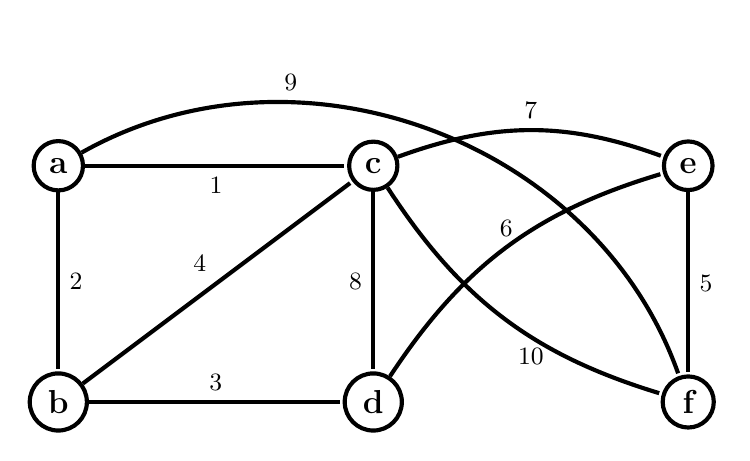
\begin{tikzpicture}[-,>=stealth,shorten >=1pt,auto,
  main node/.style={circle,draw,font=\large\bfseries}, line width=1.5pt]
\node[main node] (a) at (1,1.5) {a};
\node[main node] (b) at (1,-1.5) {b};
\node[main node] (c) at (5,1.5) {c};
\node[main node] (d) at (5,-1.5) {d};
\node[main node] (e) at (9,1.5) {e};
\node[main node] (f) at (9,-1.5) {f};

\path[every node/.style={font=\small}]
(a) edge node {2} (b)
(a) edge[below] node {1} (c)
(a) edge[bend left=50] node[pos=.3, above] {9} (f)
(b) edge node {3} (d)
(b) edge node {4} (c)
(c) edge[left] node {8} (d)
(c) edge[above,bend left=20] node {7} (e)
(d) edge[above,bend left=20] node {6} (e)
(e) edge node {5} (f)
(c) edge[below, bend right=20] node[pos=.6] {10} (f);
\end{tikzpicture}
\end{center}

Which edges are in the minimum spanning tree?
\multipleanswers
\optionsstart
\answer \{a,b\} \correct
\answer \{a,c\} \correct
\answer \{a,f\}
\answer \{b,c\}
\answer \{b,d\} \correct
\answer \{c,d\}
\answer \{c,e\}
\answer \{c,f\}
\answer \{d,e\} \correct
\answer \{e,f\} \correct
\optionsend

\explanation{
Run Kruskal's algorithm: sort the edges by weight and add each one if it does not form a cycle.
First \{a,c\} (1), \{a,b\} (2), \{b,d\} (3) are added. The edge \{b,c\} (4) is skipped, since it would create the cycle a--b--c--a.
Then \{e,f\} (5) and \{d,e\} (6) are added, which connects the two components and gives a spanning tree.
}



\question{Shortest paths}
Consider the following weighted, directed graph:
\begin{center}
  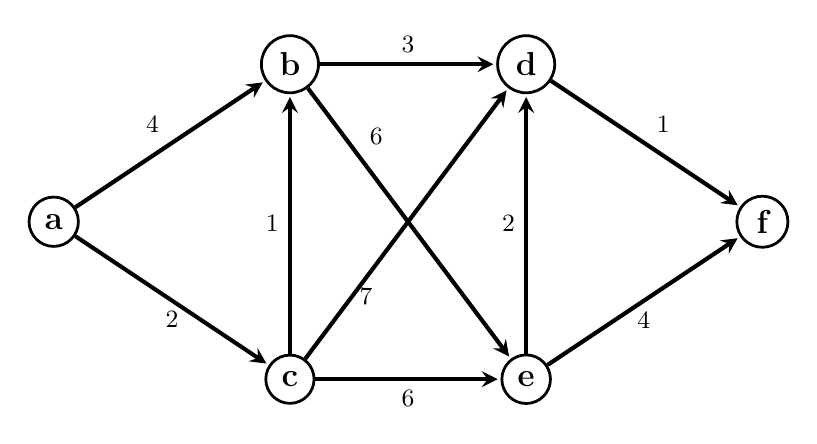
\begin{tikzpicture}[->,>=stealth,shorten >=1pt,auto,
      main node/.style={circle,draw,font=\large\bfseries,line width=1pt}, line width=1.5pt]
  \node[main node] (a) at (0,0) {a};
  \node[main node] (b) at (3,2) {b};
  \node[main node] (c) at (3,-2) {c};
  \node[main node] (d) at (6,2) {d};
  \node[main node] (e) at (6,-2) {e};
  \node[main node] (f) at (9,0) {f};
  \path[every node/.style={font=\small}]
  (a) edge node {4} (b)
  (a) edge[below] node {2} (c)
  (c) edge node {1} (b)
  (c) edge[below] node {6} (e)
  (c) edge node[pos=.3,below] {7} (d)
  (b) edge node {3} (d)
  (b) edge node[pos=.25] {6} (e)
  (e) edge node {2} (d)
  (d) edge node {1} (f)
  (e) edge[below] node {4} (f);
  \end{tikzpicture}
\end{center}

Suppose Dijkstra's algorithm is run with source vertex {\bf a}.
In which order are the vertices extracted from the priority queue?
\oneanswer
\optionsstart
\answer a, c, b, d, e, f
\answer a, c, b, d, f, e \correct
\answer a, c, b, e, f, d
\answer a, c, b, e, d, f
\answer a, c, b, f, d, e
\answer a, c, b, f, e, d
\optionsend

\explanation{
From the source vertex {\bf a} we first get the distances $d[b]=4$ and $d[c]=2$.
Therefore {\bf c} is extracted next.
The edge $({\bf c},{\bf b})$ improves the distance to {\bf b} to $3$, so {\bf b} is extracted before the remaining vertices.
Next, the edge $({\bf b},{\bf d})$ improves the distance to {\bf d} to $6$, while {\bf e} has distance $8$ via {\bf c}.
Therefore {\bf d} is extracted before {\bf e}.
The edge $({\bf d},{\bf f})$ gives $d[f]=7$, so {\bf f} is extracted before {\bf e}.
The order is therefore a, c, b, d, f, e.
}



\question{Activity selection}
Consider {\sc Greedy-Activity-Selector} from CLRS Section 15.1. What result does the algorithm return on the following input, where the activities are already sorted by finish time:
s = $\langle 1,3,0,5,8,5\rangle$ and f = $\langle 2,4,6,7,9,9\rangle$?
\oneanswer
\optionsstart
\answer A = $\langle a_1,a_2,a_4,a_5\rangle$ \correct
\answer A = $\langle a_1,a_2,a_5,a_6\rangle$
\answer A = $\langle a_1,a_3,a_4,a_5\rangle$
\answer A = $\langle a_1,a_3,a_5,a_6\rangle$
\optionsend
\explanation{Running the algorithm by hand gives the answer shown. Moreover, the other possible answers do not satisfy the condition that the activities must be disjoint.
}




\question{Longest common subsequence}
The strings {\tt BANANA} and {\tt ANAGRAM} both have the subsequence {\tt ANAA}, and it is a longest common subsequence.
How many different common subsequences of length 4 are there?
\oneanswer
\optionsstart
\answer 1 \correct
\answer 2
\answer 3
\answer 4
\optionsend
\explanation{The characters G, R and M occur in only one of the strings and are therefore never part of a common subsequence. We can therefore restrict our attention to common subsequences of {\tt BANANA} and {\tt ANAA}, and it is clear that only one of them has length 4.

Alternatively (more generally): The LCS algorithm makes an arbitrary choice when the cells to the left and above in the dynamic programming table contain the same value. These cases are marked for our input in the table below:
\begin{center}
\begin{tabular}{c|c|c|c|c|c|c|c|c||}
    &   & A & N & A & G & R & A & M\\
    \hline
     & 0 & 0 & 0 & 0 & 0 & 0 & 0 & 0\\
     \hline
    B & 0 & $\uparrow0$ & $\uparrow0$ & $\uparrow0$ & $\uparrow0$ & $\uparrow0$ & $\uparrow0$ & $\uparrow0$ \\
    A & 0 & $\nwarrow1$ & $\leftarrow1$ & $\nwarrow1$ & $\leftarrow1$ & $\leftarrow1$ & $\nwarrow1$ & $\leftarrow1$ \\
    N & 0 & $\uparrow1$ & $\nwarrow2$ & $\leftarrow2$ & $\leftarrow2$ & $\leftarrow2$ & $\leftarrow2$ & $\leftarrow2$ \\
    A & 0 & $\nwarrow1$ & $\uparrow2$ & $\nwarrow3$ & $\leftarrow3$ & $\leftarrow3$ & $\nwarrow3$ & $\leftarrow3$ \\
    N & 0 & $\uparrow1$ & $\nwarrow2$ & $\uparrow3$ & $\color{red}\uparrow3$ & $\color{red}\uparrow3$ & $\uparrow3$ & $\uparrow3$ \\
    A & 0 & $\nwarrow1$ & $\uparrow2$ & $\nwarrow3$ & $\uparrow3$ & $\uparrow3$ & $\nwarrow4$ & $\leftarrow4$ \\
    \hline
\end{tabular}
\end{center}
\noindent
We see that even if we had chosen $\leftarrow$ instead of $\uparrow$ (where the value is 3) in one or more of these steps, the output would still be {\tt ANAA}. Therefore {\tt ANAA} is the only longest common subsequence.
}




\question{Parallel algorithms}
Suppose that a parallel algorithm on inputs of size $n$ has work $T_1=\Theta(n^2)$ and span $T_\infty=\Theta(n)$.
We are interested in the time $T_P$ used to run the algorithm on $P$ processors with greedy scheduling.
Which of the statements below are correct?
\multipleanswers
\optionsstart
\answer If $P=\Theta(1)$ then $T_P=O(n^2)$ \correct
\answer If $P=\Theta(\log n)$ then $T_P=O(n \log n)$
\answer If $P=\Theta(n)$ then $T_P=O(n)$ \correct
\answer If $P=\Theta(n^2/\log n)$ then $T_P=O(\log n)$
\answer If $P=\Theta(n^2)$ then $T_P=O(1)$
\optionsend
\explanation{By CLRS Theorem 26.1, $T_P \leq T_1 / P + T_\infty$, and by Theorem 26.2 this bound is within a factor 2 of the true running time.
Substituting the given values of $P$ yields:
\begin{align*}
P=\Theta(1) &: \quad T_P=\Theta(n^2+n)=\Theta(n^2) \text{ which is } O(n^2),\\[4pt]
P=\Theta(\log n) &: \quad
T_P=\Theta\left(\frac{n^2}{\log n}+n\right)
=\Theta\!\left(\frac{n^2}{\log n}\right)\text{ which is not } O(n\log n),\\[4pt]
P=\Theta(n) &: \quad T_P=\Theta(n+n)=\Theta(n) \text{ which is } O(n),\\[4pt]
P=\Theta(n^2/\log n) &: \quad
T_P=\Theta(\log n+n)=\Theta(n) \text{ which is not } O(\log n),\\[4pt]
P=\Theta(n^2) &: \quad
T_P=\Theta(1+n)=\Theta(n) \text{ which is not } O(1).
\end{align*}
}



% Let $G = (V,E)$ be a connected simple graph with $|V|=n$ and let $w : E \to \mathbb{N}$ be an edge-weight function. Assume that all weights are distinct (that is, $w$ is an injection). Denote by $M$ the number of minimum spanning trees in $G$ with respect to $w$. Which of the following is always true?

\question{Minimum spanning trees}
Let $G = (V,E)$ be a connected, simple graph with $|V|=n$, and let $w : E \to \mathbb{R}$ be an edge-weight function.
Assume that all weights are distinct (i.e.,~that $w$ is injective).
Denote by $M$ the number of distinct minimum spanning trees in $G$ with respect to $w$.
Which of the following statements are always true, regardless of the choice of $G$ and $w$?
\multipleanswers
Note that some of the statements are related in the sense that if one of them always holds, then the other one also always holds.
\optionsstart
\answer $M \geq 1$ \correct
\answer $M \leq 1$ \correct
\answer $M \geq n$
\answer $M \leq n$ \correct
\answer None of the above statements are always true.
\optionsend
\explanation{
% The answer is $M=1$.
% If two different MSTs exist, replace the smallest-weight edge that appears in one but not the other.
There is always exactly one minimum spanning tree when all weights are distinct.
If there were two different minimum spanning trees, one could consider the edge of minimum weight that appears in one tree but not in the other, and use the cut property to derive a contradiction. Therefore all of the inequalities are true except $M \geq n$.
}



%Let $T$ be a tree with $n>4$ vertices that is a tree-path going to the right.
%Here is an illustration with 9 vertices.

\question{Balancing search trees}
For an odd integer $n$, let $T$ be a highly unbalanced binary search tree with $n$ keys and $(n+1)/2$ nodes on a path going to the right.
Below is an illustration with $n=9$ keys and a path of length~5.

\begin{center}
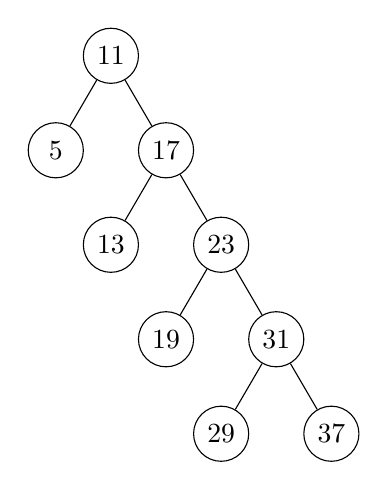
\begin{tikzpicture}[
  every node/.style={
    circle,
    draw,
    minimum size=7mm,
    inner sep=1pt
  },
  edge from parent/.style={draw},
  level distance=12mm,
  sibling distance=14mm
]

\node {11}
  child { node {5} }
  child { node {17}
    child { node {13} }
    child { node {23}
      child { node {19} }
      child { node {31}
        child { node {29} }
        child { node {37} }
      }
    }
  };
\end{tikzpicture}
\end{center}
%Using asymptotic notation, what is the minimum number of rotations needed to change the tree to have depth at most $10 \log_2(n)$?
What is the minimum number of rotations that must be performed to change $T$ so that it has depth at most $10 \log_2(n)$?
We are interested in the answer for large values of $n$, expressed using asymptotic notation.
\oneanswer
\optionsstart
\answer $\Theta(n)$ \correct
\answer $\Theta(n \log n)$
\answer $\Theta(n^2)$
\answer $\Theta(n^2 \log n)$
\optionsend
\explanation{
% The answer is $\Theta(n)$. For the upper bound, which is the relevant part for the question, perform the balancing in iterations. In each iteration, left-rotate every second node. After $k$ iterations, every subtree hanging off the current ``right spine'' has height at most $k$.
% And the length of the ``right spine'' becomes $O(n/2^k)$.
Each rotation can reduce the depth by at most 1, so at least $\Omega(n)$ rotations are required.
We argue that $O(n)$ rotations suffice:
The rotations can be performed in iterations, where each iteration performs a left rotation at every second node on the path going to the right, e.g., 17 and 31 in the example.
This reduces the length of the path by a factor of 2.
After $k$ iterations, every subtree hanging to the left of the right path has height at most $k$.
Therefore the depth of the tree becomes at most $O(n/2^k + k)$.
After $k=\log_2(n)$ iterations the depth of the tree is at most $2\log_2(n)$.
The number of rotations in iteration $k$ is $\Theta(n/2^k)$, so the total number of rotations is $\Theta(\sum_{k=1}^{\lg n} n/2^k)$, which is $\Theta(n)$.
}

\question{Graham's Scan}
Consider the following set of points.

\begin{center}
\begin{tikzpicture}[scale=0.75]
  \draw[->] (-0.3,0) -- (5.8,0) node[right] {$x$};
  \draw[->] (0,-0.3) -- (0,5.8) node[above] {$y$};

  \foreach \x/\y/\name in {
    0/0/p_0,
    4/0/p_1,
    2/1/p_2,
    5/3/p_3,
    2/2/p_4,
    3/5/p_5,
    1/4/p_6
  }{
    \fill (\x,\y) circle (2pt);
    \node[above right] at (\x,\y) {$\name$};
  }
\end{tikzpicture}
\end{center}

Suppose \proc{Graham-Scan} (CLRS online Chapter 33) is run on the set of points. The points are numbered as in the algorithm, so $p_0$ is the leftmost of those with minimum $y$-coordinate, and the others are sorted by polar angle
around $p_0$ in the order
\[
p_1,p_2,p_3,p_4,p_5,p_6.
\]
The stack $S$ is written from bottom to top.
Which of the following are identical to the contents of the stack $S$ at some point while the algorithm runs?
(Note that the question is \emph{not} which points are on the stack at some point.)
\multipleanswers

\optionsstart
\answer{$\langle p_0,p_1,p_2,p_3,p_4,p_5\rangle$}
\answer{$\langle p_0,p_1,p_3,p_4,p_5\rangle$}
\answer{$\langle p_0,p_1,p_3,p_5\rangle$}\correct
\answer{$\langle p_0,p_2,p_3,p_5\rangle$}
\answer{$\langle p_0,p_2,p_1\rangle$}
\answer{$\langle p_0,p_2,p_5,p_6\rangle$}
\optionsend

\explanation{
After the initialization in lines 6--8 the stack is
\(
\langle p_0,p_1,p_2\rangle
\).
When $p_3$ is processed, $p_1,p_2,p_3$ form a non-left turn, so
$p_2$ is popped. Then $p_3$ is pushed, and the stack is
\(
\langle p_0,p_1,p_3\rangle
\).
When $p_4$ is processed, it is pushed without any points being popped:
\(
\langle p_0,p_1,p_3,p_4\rangle
\).
When $p_5$ is processed, $p_3,p_4,p_5$ form a non-left turn, so
$p_4$ is popped. Then $p_5$ is pushed, and the stack is therefore
\(
\langle p_0,p_1,p_3,p_5\rangle
\).
The other answers do not occur. % for various reasons
}


% Let $G$ be the bipartite graph with two sides $L = \{\ell_1,\ldots,\ell_{10}\}$ and $R = \{r_1,\ldots,r_{10}\}$.
% The edges of $G$ are defined as follows: there is an edge between $\ell_i$ and $r_j$ if and only if $i \leq j$.
% Denote by $N$ the number of perfect matchings in $G$.
% Which of the following is true?

\question{Perfect matching}
Let $G$ be a bipartite graph with vertex sets $L = \{\ell_1,\ldots,\ell_{10}\}$ and $R = \{r_1,\ldots,r_{10}\}$ where
there is an edge between $\ell_i$ and $r_j$ if and only if $i \leq j$.
Denote by $N$ the number of perfect matchings in $G$.
Which of the following statements is true?
\oneanswer
\optionsstart
\answer $N=0$
\answer $N=1$ \correct
\answer $N=2$
\answer $N=10$
\answer $N = {10 \choose 2}$
\optionsend
\explanation{
% There is a single perfect matching. Every permutation $\pi$ that is not the identity maps some $i$ to $\pi(i) < i$ so it is not in the graph. The identity matching is present.
Every permutation $\pi: \{1,\dots,10\} \to \{1,\dots,10\}$ that is not the identity function has an input $i$ with $\pi(i)<i$, so the corresponding matching does not exist in the graph.
So the only matching is the one corresponding to the identity function.
}


\multiplechoiceend

\newpage

\section*{Written problems}\label{sec:written}

% Machine translated from the Danish original, ../danish/skriftlige.tex
{\bf Written problems:} \placeholder{How the answers are submitted, e.g.\ the file format and exam system, and whether drawings made on a tablet may be inserted.}
\begin{itemize}
    \item Use \emph{one page for each subquestion, in the same order as in the problem set.}
    \item The number/letter of the subquestion (e.g.\ 19 or 20.a) must be stated.
\end{itemize}



\section{Insertion into a red-black search tree (4\%)}
We start with an empty red-black binary search tree.
Insert the keys
\[
30,15,45,10
\]
in the given order using the CLRS algorithm {\sc RB-Insert}.

\subquestion{}{Draw the resulting red-black search tree, indicating the color of each node.}

\explanation{
After inserting 30, the node becomes the root and is colored black.
The keys 15 and 45 are inserted as red children of 30.
The key 10 is inserted as a red left child of 15.
Since both 15 and its sibling 45 are red, 15 and 45 are recolored black, and 30 is temporarily recolored red, after which the root is colored black again.
The resulting tree is:
\begin{center}
\begin{tikzpicture}[-,>=stealth,level/.style={sibling distance = 4cm/#1,
    level distance = 1cm}, line width=1.5pt]
  \node [black] {30}
      child{ node [black] {15}
              child{ node [red] {10} }
              child[missing]
      }
      child{ node [black] {45} };
\end{tikzpicture}
\end{center}
}


\section{Interval covering (12\%)}

We are given a number $L>0$ and a collection of $n$ intervals
\[
I_i=[a_i,b_i],
\]
where $i\in\{1,2,\ldots,n\}$ and $a_i < b_i$.
We want to select as few intervals as possible such that their union covers the entire interval $[0,L]$.
That is, we want to find $J\subseteq\{1,2,\ldots,n\}$ such that $[0,L]\subseteq\bigcup_{i\in J} I_i$ and $\vert J\vert$ is as small as possible.
The algorithm must return the size $\vert J\vert$.

\subquestion{a)}
{Let $L=12$, and let the intervals be
\[
[2,8],\ [-1,4],\ [1,5],\ [8,12],\ [6,20],\ [7,9].
\]
Give an optimal solution and briefly justify your answer.}

\explanation{
An optimal solution is, e.g.,
\[
[-1,4],\ [2,8],\ [6,20].
\]
(Another valid choice is $[-1,4]$, $[2,8]$, $[8,12]$).
These three intervals cover all of $[0,12]$.
There is no solution with only two intervals: To cover $0$ we must use $[-1,4]$, and no single interval covers all the way from $4$ to $12$.
Therefore three intervals is optimal.
}


\subquestion{b)}
{Describe an efficient algorithm that finds a minimum number of intervals covering $[0,L]$, if such a cover exists.
If $[0,L]$ cannot be covered, the algorithm must return \const{false}.
The input to the algorithm is $(a,b,n,L)$, where $a[1{:}n]$ and $b[1{:}n]$ are arrays of length $n$ containing the start and end points, i.e.,~$I_i=[a[i],b[i]]$.
You may write pseudocode, but a clear and precise description in prose is also sufficient.
You must account for the running time of the algorithm -- to get full points it must be $O(n\log n)$.}

\explanation{
First sort the intervals by left endpoint.
We maintain a variable $x$ indicating that we have already covered $[0,x]$.
Initially $x=0$.
As long as $x<L$, we scan all intervals that start at or before $x$, and among these find the interval that reaches farthest to the right.
If no such interval reaches beyond $x$, then $[0,L]$ cannot be covered.
Otherwise we select the interval and update $x$.
To scan the intervals efficiently, we maintain an index $i$, so that we can start the search from the most recently added interval.

\begin{codebox}
\Procname{$\proc{CoverInterval}(a,b,n,L)$}
\li sort the intervals by increasing $a[i]$
\li $x \gets 0$
\li $i \gets 1$
\li $k \gets 0$
\li \While $x < L$
\Do
\li     $best \gets x$
\li     \While $i \le n$ \textbf{and} $a[i] \le x$
\Do
\li         \If $b[i] > best$
\li         \Then $best \gets b[i]$
            \End
\li         $i \gets i+1$
        \End
\li     \If $best == x$
\li     \Then \Return \const{false}
        \End
\li     $x \gets best$
\li     $k \gets k+1$
    \End
\li \Return $k$
\end{codebox}

Sorting takes $O(n\log n)$ time.
After sorting, each interval is processed at most once in the inner while loop, so the rest of the algorithm takes $O(n)$ time.
The total running time is therefore $O(n\log n)$.
}

\subquestion{c)}
{Argue that the algorithm always finds a minimum number of intervals, if a cover exists.}

\explanation{
We show that the greedy choice is safe.
Suppose that at some point the algorithm has covered the interval $[0,x]$.
Any valid solution to the rest of the problem must use an interval $I_i$ that starts at or before $x$, since otherwise there would be a gap in the cover.
Among all such intervals, the algorithm selects an interval $I_{i^*}$ that reaches as far to the right as possible.
If $I_i$ and $I_{i^*}$ are different intervals, we could replace $I_i$ by $I_{i^*}$ and still have a valid solution, since $b[i^*]\geq b[i]$.

By induction on the number of intervals, it follows that the algorithm's choice in each step can be part of an optimal solution.
The algorithm therefore finds the smallest possible number of intervals.
}


\section{Increasing polygonal chain (12\%)}\label{sec:last}

We are given $n$ points in the plane
\(
p_i=(x_i,y_i),
\)
where $i\in\{1,2,\ldots,n\}$.
We assume that all $x_i$-coordinates are distinct.
%
An increasing polygonal chain is a sequence of points
\[
p_{i_1},p_{i_2},\ldots,p_{i_k}
\]
such that
\[
x_{i_1}<x_{i_2}<\cdots <x_{i_k}
\text{ and }
y_{i_1}<y_{i_2}<\cdots <y_{i_k} \enspace .
\]
Consider the problem of finding the length $k$ of a longest possible increasing polygonal chain.
Below is an example of a set of points and an increasing chain of length 3, illustrated as a path (not necessarily the longest).

\begin{center}
\begin{tikzpicture}[scale=0.75]
  \draw[->] (0,0) -- (9,0) node[right] {$x$};
  \draw[->] (0,0) -- (0,7) node[above] {$y$};

  \foreach \x/\y/\name in {
    1/2/$p_1$,
    2/5/$p_2$,
    3/3/$p_3$,
    4/6/$p_4$,
    5/4/$p_5$,
    6/5/$p_6$,
    7/2/$p_7$,
    8/6/$p_8$
  } {
    \fill (\x,\y) circle (2pt);
    \node[above right] at (\x,\y) {\name};
  }

  \draw[thick] (1,2) -- (2,5) -- (4,6);
\end{tikzpicture}
\end{center}

\subquestion{a)}
{Consider the points shown in the figure above, i.e.,
\[
\begin{array}{c|cccccccc}
i    & 1&2&3&4&5&6&7&8\\ \hline
x_i  & 1&2&3&4&5&6&7&8\\
y_i  & 2&5&3&6&4&5&2&6
\end{array}
\]
Give a longest possible increasing polygonal chain.}

\explanation{
A longest possible increasing polygonal chain is
\[
p_1,p_3,p_5,p_6,p_8.
\]
It has length $5$ and is increasing, since
\(
2<3<4<5<6
\)
for the $y$-coordinates, and the points are already in increasing order of $x$-coordinate.
}

\subquestion{b)}
{Describe an efficient algorithm that finds the length of a longest possible increasing polygonal chain.
The input to the algorithm is arrays $x[1{:}n]$ and $y[1{:}n]$ of length $n$, where point $i$ is $(x[i],y[i])$.
You must account for the running time of the algorithm -- to get full points it must be $O(n^2)$.}

\explanation{
First sort the points by increasing $x$-coordinate.
Let $D[i]$ be the length of a longest possible increasing chain ending at point $i$.
Then
\[
D[i] =
\begin{cases}
1, & \text{if there is no } j<i \text{ with } y[j]<y[i],\\
1+\max\{D[j]\mid j<i \text{ and } y[j]<y[i]\}, & \text{otherwise.}
\end{cases}
\]

\begin{codebox}
\Procname{$\proc{IncreasingChain}(x,y,n)$}
\li sort the points by increasing $x[i]$
\li \For $i \gets 1$ \To $n$
\Do
\li     $D[i] \gets 1$
\li     \For $j \gets 1$ \To $i-1$
\Do
\li         \If $y[j] < y[i]$
\li         \Then $D[i] \gets \max(D[i],D[j]+1)$
            \End
        \End
    \End
\li \Return $\max_{1\le i\le n} D[i]$
\end{codebox}

Sorting takes $O(n\log n)$ time.
The two loops take $O(n^2)$ time.
The total running time is therefore $O(n^2)$.
}

\subquestion{c)}
{Argue that the algorithm always finds the length of a longest possible increasing polygonal chain.}

\explanation{
Consider a longest possible increasing chain ending at point $i$.
If the chain consists only of point $i$, it has length $1$.
Otherwise the second-to-last point must be a point $j$ with $j<i$ and $y[j]<y[i]$.
The best chain ending at $i$ is therefore obtained by taking the best chain ending at such a point $j$ and appending point $i$.

This is exactly what the recurrence for $D[i]$ computes.
Since the values $D[j]$ for $j<i$ have already been computed when $D[i]$ is computed, correctness follows by induction on $i$.
Finally, an optimal chain can end at any point, so the algorithm returns $\max_i D[i]$.
}

\label{page:last}
